\chapter{Defects}

\label{ch:defects}

\section{Frenkel and Schottky defects}

\subsection{Incorporation and defect formation energies}

\subsubsection*{Isolated Frenkel defects}

Zr and O Frenkel pair defect formation energies were determined via point defect DFT calculations for the three structures. The formation energies of the isolated Frenkel defect pairs were defined as:
% Interstitial iodine defects were simulated in the neutral charge state at different interstitial sites in each phase. The incorporation energy of these defects, assuming a perfect lattice, was calculated using Equation \ref{equation_incorporation}:

\begin{equation}
\label{equation_frenkel}
E_{Frenkel} = E_{DFT}(V^{q}_{X}) + E_{DFT}(X^{-q}_{i}) - 2E_{DFT}(ZrO_2)% - \frac{E_{I_2}}{2}
\end{equation}

where $X$ is either Zr or O, $E_{DFT}(V^{q}_{X})$ is the energy of a supercell of \zirconia\ containing a single vacancy of charge $q$, $E_{DFT}(X^{-q}_{i})$ is the energy of a supercell of \zirconia\ containing a single interstitial with opposing charge $-q$, and $E_{DFT}(ZrO_2)$ is the energy of the non-defective supercell. Charges ranged from the fully charged case (+2 for oxygen vacancies, -4 for zirconium vacancies) to neutral. The interstitial sites, shown in Table \ref{table:interstitials}, were chosen based on standard vacant Wyckoff positions in each crystal structure \cite{theo1996international}.  In the case of oxygen vacancies in monoclinic \zirconia , a defect energy was obtained for both the (III) and (IV) co-ordinated oxygen sites, with the lowest energy value being used in the calculation of the Frenkel defect energy.

\begin{table}[ht] % Wyckoff positions of interstitials
\onehalfspacing
\centering
\caption{Wyckoff positions of interstitial sites used for each crystal structure.}
\label{table:interstitials}
\begin{tabular}{lcc}
\hline
\hspace{0.7 cm} {\bf Crystal Structure} \hspace{0.7 cm}                              & \hspace{0.7 cm} {\bf Interstitial Sites} \hspace{0.7 cm}                                               \\ \hline
\multicolumn{1}{c}{\textbf{Monoclinic}}              & $2a$, $2b$, $2c$, $2d$ \\
\multicolumn{1}{c}{\textbf{Tetragonal}}            & $2b$, $8e$                                   \\
\multicolumn{1}{c}{\textbf{Cubic}}       & $24d$, $4b$                                          \\ \hline
\end{tabular}
\end{table}

The isolated defect formation energies reported in Table \ref{isolated_defects} indicate that fully-charged Schottky defects have the lowest formation energy per atom (most energetically favourable) in all phases, followed by oxygen Frenkel defects and then zirconium Frenkel defects. A trend is seen where the high-temperature phases result in lower formation energies for both Schottky and oxygen Frenkel defects, whereas zirconium Frenkel defects have similar formation energies in all three phases. 

It has been suggested that the relatively small cation size leads to defect structures where oxygen vacancies are favoured over interstitial defects \cite{dwivedi1990computer}. As the zirconium ion is too small to maintain a strong 8-fold bond coordination with its neighbouring oxygen ions, the introduction of oxygen vacancies (which have the added effect of reducing cell volume) will have a stabilising effect.

\begin{table}[ht] % Isolated formation energies
\onehalfspacing
\centering
\caption{Formation energies in eV of isolated \zirconia\ defects.}
\label{isolated_defects}
\begin{tabular}{cccll}
\hline
\multirow{2}{*}{\textbf{Defect}}                      & \multirow{2}{*}{\textbf{Equation}}                                        & \multicolumn{3}{c}{\textbf{Formation Energy (eV)}} \\ \cline{3-5}
	&	& \multicolumn{1}{l}{Monoclinic} & Tetragonal & Cubic \\ \hline
\multirow{5}{*}{\textbf{Zr Frenkel}} & \ch{Zr_{Zr}^{x}} $\rightarrow$ \ch{V_{Zr}^{''''}} + \ch{Zr_{i}^{****}}              & 5.428 & 5.639 & 5.610                             \\
                                     & \ch{Zr_{Zr}^{x}} $\rightarrow$ \ch{V_{Zr}^{'''}} + \ch{Zr_{i}^{***}}               & 8.695 & 8.939 & 8.476                            \\
                                     & \ch{Zr_{Zr}^{x}} $\rightarrow$ \ch{V_{Zr}^{''}} + \ch{Zr_{i}^{**}}                & 12.118 & 12.058 & 11.628                             \\
                                     & \ch{Zr_{Zr}^{x}} $\rightarrow$ \ch{V_{Zr}^{'}} + \ch{Zr_{i}^{*}}                & 16.021 &	15.696 &	13.319                             \\
                                     & \ch{Zr_{Zr}^{x}} $\rightarrow$ \ch{V_{Zr}^{x}} + \ch{Zr_{i}^{x}}                  & 20.563	& 20.094 &	18.170                            \\ \hline
\multirow{3}{*}{\textbf{O Frenkel}}  & \ch{O_{O}^{x}} $\rightarrow$ \ch{V_{O}^{**}} + \ch{O_{i}^{''}}                   & 4.457 &	4.000 & 	3.728                             \\
                                     & \ch{O_{O}^{x}} $\rightarrow$ \ch{V_{O}^{*}} + \ch{O_{i}^{'}}                   & 6.432	& 6.588 &	7.055                             \\
                                     & \ch{O_{O}^{x}} $\rightarrow$ \ch{V_{O}^{x}} + \ch{O_{i}^{x}}                     & 7.518 &	7.452 &	8.477                             \\ \hline
\multirow{3}{*}{\textbf{Schottky}}   & $\varnothing$ $\rightarrow$ \ch{V_{Zr}^{''''}} + 2\ch{V_{O}^{**}} & 5.120 &	3.778	& 1.752                             \\
                                     & $\varnothing$ $\rightarrow$ \ch{V_{Zr}^{''}} + 2\ch{V_{O}^{*}} & 11.353 &	10.832 &	9.624                             \\
                                     & $\varnothing$ $\rightarrow$ \ch{V_{Zr}^{x}} + 2\ch{V_{O}^{x}}   & 18.554 &	18.232 &	17.073  \\ \hline                          
\end{tabular}
\end{table}

\subsubsection*{Bound Frenkel Defects}

Bound Zr and O Frenkel defect formation energies were calculated from DFT energies of supercells where a single ion was moved from its lattice site to an interstitial site. The formation energies of the bound Frenkel defect pairs were defined as:
% Interstitial iodine defects were simulated in the neutral charge state at different interstitial sites in each phase. The incorporation energy of these defects, assuming a perfect lattice, was calculated using Equation \ref{equation_incorporation}:

\begin{equation}
\label{equation_frenkel_bound}
E_{BoundFrenkel} = E_{DFT}(BoundFrenkel) - E_{DFT}(ZrO_2)% - \frac{E_{I_2}}{2}
\end{equation}

where $E_{DFT}(BoundFrenkel)$ is the energy of a supercell of \zirconia\ containing both a vacancy and interstitial defect of the same ion. The two defects were placed as far apart in the supercell as possible (7-8 \r{A}) to avoid recombination. The interstitial defect is assumed to fully compensate the charge of the vacancy defect, resulting in no overall charge on the supercell. The number and type of ions in the defective and non-defective supercell are the same, requiring no further steps to calculate the formation energy. The formation energies calculated for these defects in each crystal structure are presented in Table \ref{table:bound_defects}.

\begin{table}[ht] % Bound formation energies
\onehalfspacing
\centering
\caption{Formation energies of bound defects in \zirconia.}
\label{table:bound_defects}
\begin{tabular}{cccc}
\hline
\multirow{2}{*}{\textbf{Defect}} & \multicolumn{3}{c}{\textbf{Formation Energy (eV)}} \\ \cline{2-4} 
 & \textbf{Monoclinic} & \textbf{Tetragonal} & \textbf{Cubic} \\ \hline
\textbf{O Frenkel} & 4.1212 & 4.0290 & 6.4397 \\
\textbf{Zr Frenkel} & 8.4232 & 7.8633 & 6.3274 \\
\textbf{NTV1} & 5.2272 & 3.5813 & 2.6961 \\
\textbf{NTV2} & 5.1405 & 4.2312 & 0.1798 \\
\textbf{NTV3} & 4.6620 & 3.3623 & 2.4089 \\ \hline
\end{tabular}
\end{table}

%Charges ranged from the fully charged case (+2 for oxygen, -4 for zirconium) to neutral. The interstitial sites, shown in Table \ref{table:interstitials}, were chosen based on standard vacant Wyckoff positions in each crystal structure \cite{theo1996international}.  In the case of oxygen vacancies in monoclinic \zirconia , a defect energy was obtained for both the (III) and (IV) co-ordinated oxygen sites. The lowest energies were used in the calculation of the Frenkel defect energy.

\subsubsection*{Isolated Schottky Defects}

Three Schottky energies were calculated for each structure, corresponding to fully charged, partially charged, and uncharged point defect energies. The Schottky formation energy was defined as:

\begin{equation}
\label{equation_schottky}
E_{Schottky} = E_{DFT}(V^{-2q}_{Zr}) + 2E_{DFT}(V^{q}_{O}) -\frac{3(n-1)}{n}E_{DFT}(ZrO_2)% - \frac{E_{I_2}}{2}
\end{equation}

where $n$ denotes the number of atoms in the supercell, $V^{q}_{O}$ denotes an oxygen vacancy with charge $q$, where $q$ varies from 2 to 0. This form maintains both the mass and charge balance of the Schottky defect description for \zirconia :

\begin{equation}
\label{generic_schottky}
Zr^{x}_{Zr} + 2O^{x}_{O} = V^{-2q}_{Zr} + 2V^{q}_{O} + ZrO_{2}
\end{equation}

This implies a rearrangement rather than complete removal of ions from the system. As with the Frenkel defects, the lowest energy vacancy energies were used to calculate Schottky formation energies. While there are multiple configurations of Schottky defects, such nuance cannot be accurately represented through a sum of individual vacancy defect energies. The values presented for Schottky defect formation energies should therefore be considered the lower bound for defect formation. 


\subsubsection*{Bound Schottky Defects}


\begin{figure}[ht] % Tet Zr centre
\centering
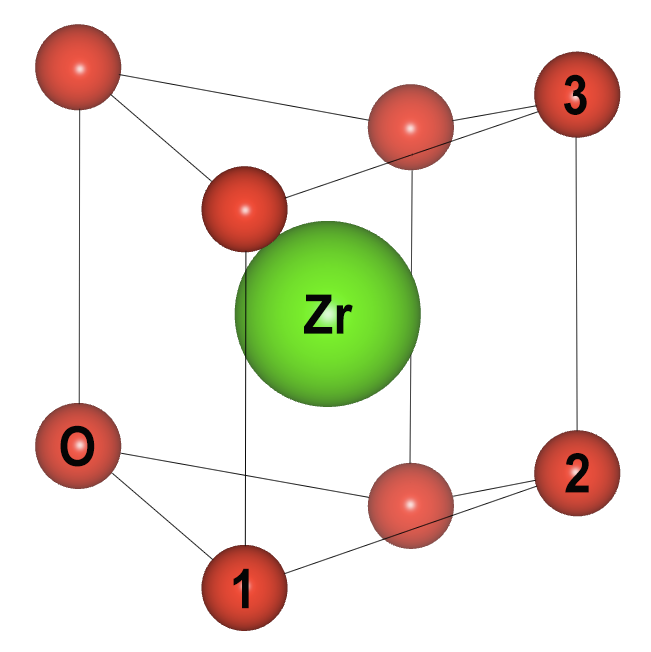
\includegraphics[width=8cm]{images/zr_centre_tet.png}
\caption{Zirconium centre unit cell showing nearest oxygen atoms in tetragonal \zirconia. Schottky trios indicated by oxygen enumeration with Zr, O and a second oxygen in either the 1\textsuperscript{st}, 2\textsuperscript{nd} or 3\textsuperscript{rd} nearest neighbour with respect to the initial oxygen. Zirconium atoms are shown in green and oxygen atoms in red.}
\label{figure:tetschottky}
\end{figure}

\begin{figure}[ht] % Cubic Zr centre
\centering
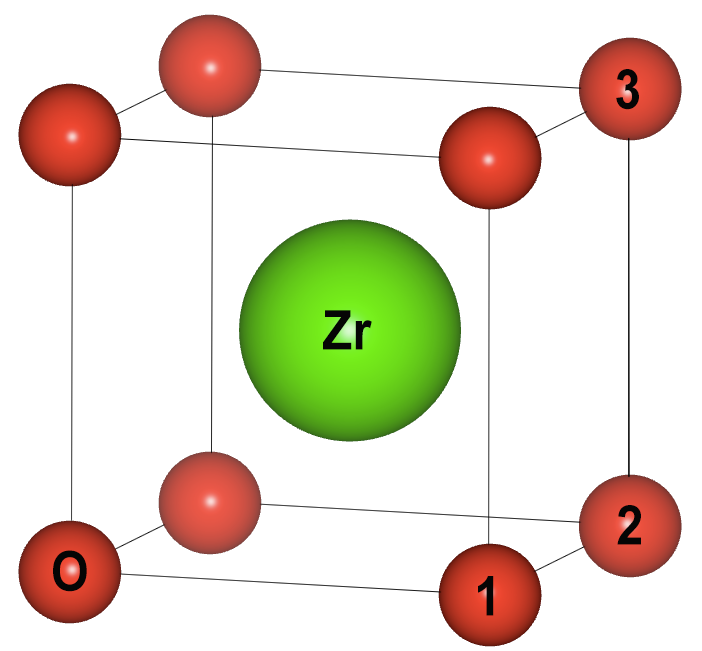
\includegraphics[width=8cm]{images/sd_cubic_zro2.png}
\caption{Zirconium centre unit cell showing nearest oxygen atoms in cubic \zirconia. Schottky trios indicated by oxygen enumeration with Zr, O and a second oxygen in either the 1\textsuperscript{st}, 2\textsuperscript{nd} or 3\textsuperscript{rd} nearest neighbour with respect to the initial oxygen.. Zirconium atoms are shown in green and oxygen atoms in red.}
\label{figure:cubicschottky}
\end{figure}

Bound Schottky defects were modelled in a supercell of \zirconia\ by removing one Zr and two O atoms, in one of several possible nearest neighbour configurations as shown in Figures \ref{figure:monoschottky}, \ref{figure:tetschottky} and \ref{figure:cubicschottky}. Charge neutrality is maintained by the removal of a stoichiometric unit, therefore these defects were defined as neutral tri-vacancies (NTVs). The NTV formation energy was defined as:

\begin{equation}
\label{equation_NTV}
E_{NTV} = E_{DFT}(NTV) - \frac{n-3}{n}E_{DFT}(ZrO_2)% - \frac{E_{I_2}}{2}
\end{equation}

Where $E_{DFT}(NTV)$ is the energy of a supercell containing the NTV defect. As the defective supercell contains three fewer ions than the non-defective cell, the energy of the non-defective cell was adjusted by a proportional factor in our calculation. This form maintains both mass and charge balance of the Schottky defect description for \zirconia\ described in Equation \ref{generic_schottky}.

\subsection{Defect formation energies}

Defect formation energies are calculated using equation \ref{equation:formation_energy}:
\begin{equation} \label{equation:formation_energy}
    E_{f} = E_{def} - E_{perf} \pm \sum_{i} n_i\mu_i + q(E_{VBM} + \mu_{e}) + E_{corr}
\end{equation}

where $E_{f}$ is the formation energy, $E_{def}$ is the energy of the defective supercell, $E_{perf}$ is the energy of a non-defective supercell, $q$ is the defect charge, $E_{VBM}$ is the valence band maximum, $\mu_{e}$ is the Fermi level and $E_{corr}$ is a charged-cell correction term.

%\section{Brouwer diagrams}
%
%\subsection{Defect equilibria}
%
%Typically in materials, several types of defects will exist simultaneously. These defects will be present at an equilibrium concentration based on their thermodynamic stability. There are several considerations to be made. In particular, it is expected that a crystal lattice will be overall charge-neutral, otherwise we would see a rapid build-up of charge with a very large Coulomb energy penalty which would be thermodynamically unsustainable.
%
%\subsection{Oxygen pressure dependence}
%
%The equilibrium concentration of defects will be a function of the oxygen partial pressure, in addition to temperature and dopant concentrations. For materials in an equilibrium state, they are necessarily in equilibrium with their surroundings. This is why even metals in evacuated vacuum flasks will produce a metal vapour pressure. In the case of \zirconia\ in nuclear fuel cladding, it is known that the ambient oxygen pressure will change over time. In particular, fission of UO$_{2}$ will result in the liberation of oxygen. This will result in an input of gaseous oxygen in the fuel cladding with increasing burn-up. The main oxygen sink is the Zr fuel cladding, into which the oxide grows. Other oxygen sinks include the oxidation of UO$_{2}$ to the oxide U$_{3}$O$_{8}$, and the oxidation of fission products. Oxidation of UO$_{2}$ is a slow process whose kinetics are largely independent of the oxygen partial pressure \cite{Desgranges2009}, and will be slowed as free space in the cladding is reduced because it results in swelling of the fuel pellet. 
